\documentclass[12pt]{standalone}
\usepackage{tikz}

\begin{document}
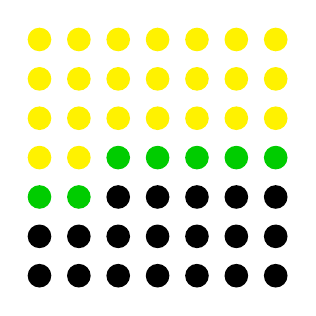
\begin{tikzpicture}[scale=0.5]
  \foreach \i in {0,...,6} {
      \foreach \j in {0,...,6} {
          \ifnum\i>3
            \fill[yellow] (\j,\i) circle (0.3);
          \else
            \ifnum\i=3
              \ifnum\j<2
                \fill[yellow] (\j,\i) circle (0.3);
              \else
                \fill[green!80!black] (\j,\i) circle (0.3);
              \fi
            \else
              \ifnum\i=2
                \ifnum\j<2
                  \fill[green!80!black] (\j,\i) circle (0.3);
                \else
                  \fill[black] (\j,\i) circle (0.3);
                \fi
              \else
                \fill[black] (\j,\i) circle (0.3);
              \fi
            \fi
          \fi
        }
    }
\end{tikzpicture}
\end{document}
